\documentclass[letterpaper,11pt,openany]{book}
\usepackage{knowledge}

\title{Элементы криптографического анализа}
\author{Автор курса: Тимонина Елена Евгеньевна \\ 
		Составитель: Смирнов Дмитрий Константинович }
\date{2022 г.}

\begin{document}

\maketitle
\tableofcontents

\mainmatter

\chapter{Домашние задания}

\section{Введение}

\section{Определение шифра. Простейшие примеры.}

\task{Что такое подстановка?}
Подстановка — это взаимно однозначная функция, которая переводит буквы алфавита в буквы того же самого алфавита.

\task{Что такое группа, и почему множество $S_m$ из примера 2.1 образует группу?}
Множество $G \ne \varnothing$ с бинарной операцией $"\circ"$, называется \emph{группой}, если выполнены условия:

1. $ \forall a,b \in G \;\; a \circ b \in G; $

2. $ \forall a,b,c \in G \;\; a \circ (b \circ c) = (a \circ b) \circ c; $

3. $ \exists e \in G \colon \forall a \in G \;\; e \circ a = a \circ e = a;$

4. $ \forall a \in G \;\; \exists b \in G \colon a \circ b = b \circ a = e$

Множество $S_m$ вводится как множество всех подстановок на конечном алфавите $A = \{a_1, ... , a_m\} $. Проверим выполнение аксиом группы:

1. Подстановка $k \in S_m$ -- отображение $k \colon A \to A$. $\forall k_1, k_2 \in S_m $ рассмотрим суперпозицию $k_1 \circ k_2$. Так как $k_1 \circ k_2 \colon A \to A \to A$, то $k_1 \circ k_2 \in S_m $ и первая аксиома верна.

2. $\forall k_1, k_2, k_3 \in S_m \;\; k_1 \circ (k_2 \circ k_3) = k_1 \circ k_2 ( k_3 (a)) = k_1 ( k_2 ( k_3 (a))) = k_1 ( k_2 (a)) \circ k_3 (a) = (k_1 \circ k_2) \circ k_3$.

3. Поскольку $S_m$ -- множество всех подстановок, то найдётся тождественная подстановка: $\exists e \in S_m \colon \forall a \in A \;\; e(a) = a$. Тогда $\forall k \in S_m $ верно $e \circ k = e(k(a)) = k(a) = k(e(a)) = k \circ e$.

4. Так как подстановка -- взаимно однозначная функция, то $\forall k \in S_m $ существует обратная функция: $\exists k^{-1} \colon A \to A \Rightarrow k^{-1} \in S_m$, для которой будет выполнено равенство $k \circ k^{-1} = k (k^{-1}(a)) = k^{-1} (k(a)) = k^{-1} \circ k$. При этом, $\forall a \in A \;\; k^{-1} (k(a)) = a = e(a)$.

Выполнены все аксиомы группы, следовательно $S_m$ -- группа.

\task{Почему группа $S_n$ из примера 2.2 является симметрической?}
Симметрической группой $n$-го порядка называется множество S(X) всех биективных отображений $f \colon X \to X$, где $X$ -- конечное множество из n элементов.
Группа $S_n$ в примере 2.2 определяется как группа подстановок на множестве $X = \{1,...,n\}$. Подстановка -- это биективное отображение, X -- конечное множество из n элементов. Следовательно, по определению, группа $S_n$ является симметрической.

\task{Что такое кольцо? Что такое кольцо вычетов по модулю $m$?}

Множество $K$ называется \emph{кольцом}, если в $K$ определены две операции $"+"$ (сложение) и $"\cdot"$ (умножение) и выполняются следующие условия $\forall a, b, c \in K$:

1. $a + b \in K, a \cdot b \in K$;

2. $a+(b+c) = (a+b)+c, \; a(bc) = (ab)c$;

3. $a+b = b+a$;

4. $(a+b)c = ac+bc$;

5. $\exists 0 \in K \colon a + 0 = a$.

Кольцом вычетов по модулю $m$ называется такое кольцо \\ $\mathbb{Z}_{/m} = \{C_0, C_1, ..., C_{m-1}\}$ ($C_r$ -- смежный класс вычетов по модулю $m$), в котором операции сложения и умножения определяются следующими правилами:

1. $C_a + C_b = C_r$, \; где $r \equiv (a+b)(\!\!\!\!\mod m)$;

2. $C_a C_b = C_r$, \; где $r \equiv ab(\!\!\!\!\mod m)$

То есть, $C_a + C_b$ -- это класс, в который входит число $a+b$, а $C_a C_b$ -- класс, в который входит число $ab$.

\task{Какую алгебраическую структуру представляет собой кольцо $\mathbb{Z}_{/m}$ при $m = 2$?}

\begin{theorem}
\label{ring_is_field}
Если $p$ -- простое число и $p \ge 2$, то $\mathbb{Z}_{/m}$ -- поле характеристики $p$.
\end{theorem}

По теореме \ref{ring_is_field} кольцо $\mathbb{Z}_{/2}$ является полем характеристики 2.


\section{Стойкость шифров. Метод полного перебора.}

\task{Дан алфавит $A = \{1,2,...,n\}$, $x$ -- открытый текст в алфавите $A$. Ключ шифрования $(T_1, T_2, T_3)$, где $T_i$ -- случайные подстановки. Алгоритм шифрования: $T_3(T_2(T_1(x))) = y$. Какова формула для расшифрования? Мощность пространства различных ключей? Сложность МПП?}

\task{Найти минимальную среднюю трудоёмкость в следующей схеме шифрования:}

{\centering
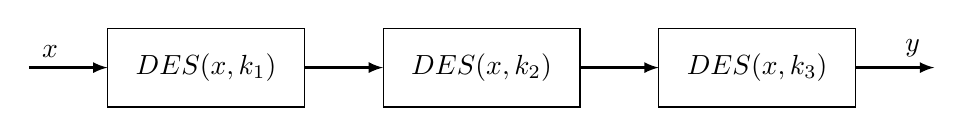
\begin{tikzpicture}[>=latex]
\draw[thick, ->] (0,0) -- node[above left] {$x$} (1,0);
\draw (1,-0.5) rectangle node[midway] {$DES(x, k_1)$} (3.5,0.5);
\draw[thick, ->] (3.5,0) -- (4.5,0);
\draw (4.5,-0.5) rectangle node[midway] {$DES(x, k_2)$} (7,0.5);
\draw[thick, ->] (7,0) -- (8,0);
\draw (8,-0.5) rectangle node[midway] {$DES(x, k_3)$} (10.5,0.5);
\draw[thick, ->] (10.5,0) -- node[above right] {$y$} (11.5,0);
\end{tikzpicture}

}

\task{В сообщении каждая буква записывается два раза. Для шифрования используется шифр перестановки длины $2n$. Сложность МПП?}

\task{}

{\centering
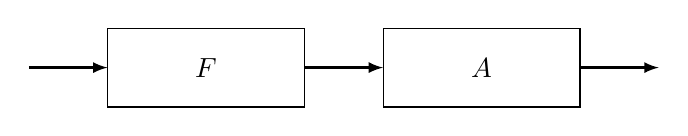
\begin{tikzpicture}[>=latex]
\draw[thick, ->] (0,0) -- (1,0);
\draw (1,-0.5) rectangle node[midway] {$F$} (3.5,0.5);
\draw[thick, ->] (3.5,0) -- (4.5,0);
\draw (4.5,-0.5) rectangle node[midway] {$A$} (7,0.5);
\draw[thick, ->] (7,0) -- (8,0);
\end{tikzpicture}

}

В данной схеме байт ОТ $x = x_1 x_2 ... x_8$ шифруется с помощью функции $F$ следующим образом:

$x_1' = x_1$;

$x_2' = x_2 + f_1(x_1)$;

$...$

$x_8' = x_8 + f_8(x_1, x_2, ..., x_7)$,

\noindent где $f_1, ..., f_7$ -- случайные булевы функции. $A$ -- невырожденная матрица. Ключом являются $F$ и $A$. Оценить сложность нахождения ключа с помощью МПП.

\task{Ключ шифрования k -- многочлен Жегалкина степени 2. Мощность пространства различных ключей? Сложность МПП?}

\task{Ключ шифрования k -- многочлен Жегалкина степени не выше $m$. Мощность пространства различных ключей? Сложность МПП?}

\task{Ключ шифрования k -- многочлен вида:
$$\sum_{1 \le i < j \le n } a_{ij} x_i x_j, a_{ij} \in \{0, 1\}.$$
Мощность пространства различных ключей? Сложность МПП?}

\end{document} 
